\documentclass[journal]{IEEEtran}
\usepackage{ctex}
\usepackage{amsmath,amsfonts,amssymb}
\usepackage{algorithmic}
\usepackage[linesnumbered,ruled]{algorithm2e}
\usepackage{array}
\usepackage{booktabs}
\usepackage{multirow}
\usepackage{tabularx}
\usepackage{graphicx}
\usepackage{cite}
\usepackage{url}
\usepackage{xcolor}
\usepackage{hyperref}
\usepackage{xcolor}
\usepackage{pgfplots}
\usepgfplotslibrary{polar}
\pgfplotsset{compat=1.18}

\definecolor{cmain}{HTML}{0178A2}
\definecolor{cwo}{HTML}{53C3C4}
\definecolor{cbase}{HTML}{EDF3F0}

\hypersetup{
  colorlinks=true,
  linkcolor=black,
  citecolor=black,
  urlcolor=black
}

\begin{document}

\title{EdgeQGFed: 面向跨模态边缘智能的质量感知云边端协同学习框架}

\maketitle

\begin{abstract}
边缘智能任务中的数据通常分散在大量弱终端上，且可能呈现图像、传感序列和网络流量等不同形态。传统联邦学习要求客户端直接训练模型，在算力、能耗、带宽和连接稳定性受限的边缘网络中代价较高。本文提出 EdgeQGFed，一种通信高效的云边端协同学习框架。客户端仅承担轻量级数据参与，边缘服务器执行主要模型更新，云端通过质量感知图注意力机制协调跨边缘知识共享。EdgeQGFed 在边缘侧结合有标签监督、云边一致性约束和置信度加权伪标签学习，以适应少标签场景；在云端融合模型表征、类别原型和训练质量信号，生成个性化边缘更新和全局教师模型。同时，框架引入资源感知客户端采样和三层通信时延模型，在通信预算、带宽异构和客户端不稳定参与条件下评估训练效率。针对网络流量五分类中的类别不均衡问题，本文进一步采用类别均衡监督和分层标注采样，提高少数类识别能力。实验覆盖图像、传感序列和网络流量任务，结果表明 EdgeQGFed 能在复杂边缘网络条件下提升模型性能、通信效率和鲁棒性。
\end{abstract}

\begin{IEEEkeywords}
边缘智能，分层联邦学习，云边端协同，图注意力，半监督学习，资源感知采样
\end{IEEEkeywords}

\section{Introduction}

大模型的发展提高了智能任务对数据、计算和模型更新能力的需求，也使训练过程更难完全依赖弱终端完成。在边缘网络中，数据持续产生于靠近用户和环境的位置。直接上传原始数据会带来通信开销和隐私风险，而让大量终端执行复杂训练又会受到算力、能耗、链路质量和连接稳定性的限制。因此，边缘智能需要一种能够将训练负载合理分配到云、边、端不同层级的协同学习机制。

联邦学习为分布式训练提供了重要思路，但传统联邦学习通常假设客户端能够周期性执行本地训练并上传模型更新。该假设在真实边缘环境中并不充分。一方面，弱客户端难以承担复杂模型训练；另一方面，链路异构、移动掉线和通信预算限制会降低训练稳定性。与此同时，边缘数据往往具有显著 non-IID 特征，且有标签样本有限。对于网络流量等类别不均衡任务，仅依赖整体准确率还可能掩盖少数类识别不足的问题。

云边端分层协同学习为上述问题提供了更可行的系统路径。客户端作为轻量级数据参与者，边缘服务器承担主要训练过程，云端负责跨边缘节点的全局协调。该范式降低了弱终端训练负担，也避免原始数据集中上传。然而，现有分层联邦方法通常将云端视为参数平均器，难以刻画不同边缘节点之间的语义关系和更新质量差异。在数据异构、标签稀缺和低质量伪标签共存的情况下，简单平均可能放大不可靠更新，引发负迁移。

为此，本文提出 EdgeQGFed，一种面向跨模态边缘智能任务的通信高效云边端协同学习框架。EdgeQGFed 将训练负载上移至边缘服务器，并利用云端计算能力对边缘节点关系进行结构化建模。云端根据模型表征、类别原型、伪标签质量、标签比例和预测置信度构建质量感知图，通过图注意力权重实现选择性知识共享。边缘侧则结合监督学习、一致性学习和伪标签学习，在少标签条件下提升训练效率。

本文进一步面向真实网络约束设计资源感知客户端采样和三层通信时延模型。客户端选择同时考虑标签比例、数据规模、带宽、掉线概率和上传时延，在通信预算下优先选择单位收益更高的参与者。对于网络流量五分类任务，本文加入类别均衡监督和分层标注采样，以缓解 R2L、U2R 等少数类识别不足。本文的主要贡献如下：

\begin{itemize}
\item [1.] 我们提出 EdgeQGFed，一种面向跨模态边缘智能任务的云边端协同学习框架，将主要训练任务上移至边缘服务器，并由云端协调跨边缘知识共享。
\item [2.] 我们设计质量感知图注意力聚合机制，融合模型表征、类别原型和训练质量信号，自适应建模边缘节点关系，缓解 non-IID 和低质量更新带来的负迁移。
\item [3.] 我们设计资源感知客户端采样与三层通信时延模型，在通信预算下联合刻画数据价值、带宽差异、掉线风险和上传时延。
\item [4.] 我们在图像、传感序列和网络流量任务上验证 EdgeQGFed，并针对类别不均衡网络流量任务引入类别均衡监督和分层标注采样。
\end{itemize}
\begin{figure}[t]
\centering

\begin{minipage}{0.241\textwidth}
\centering
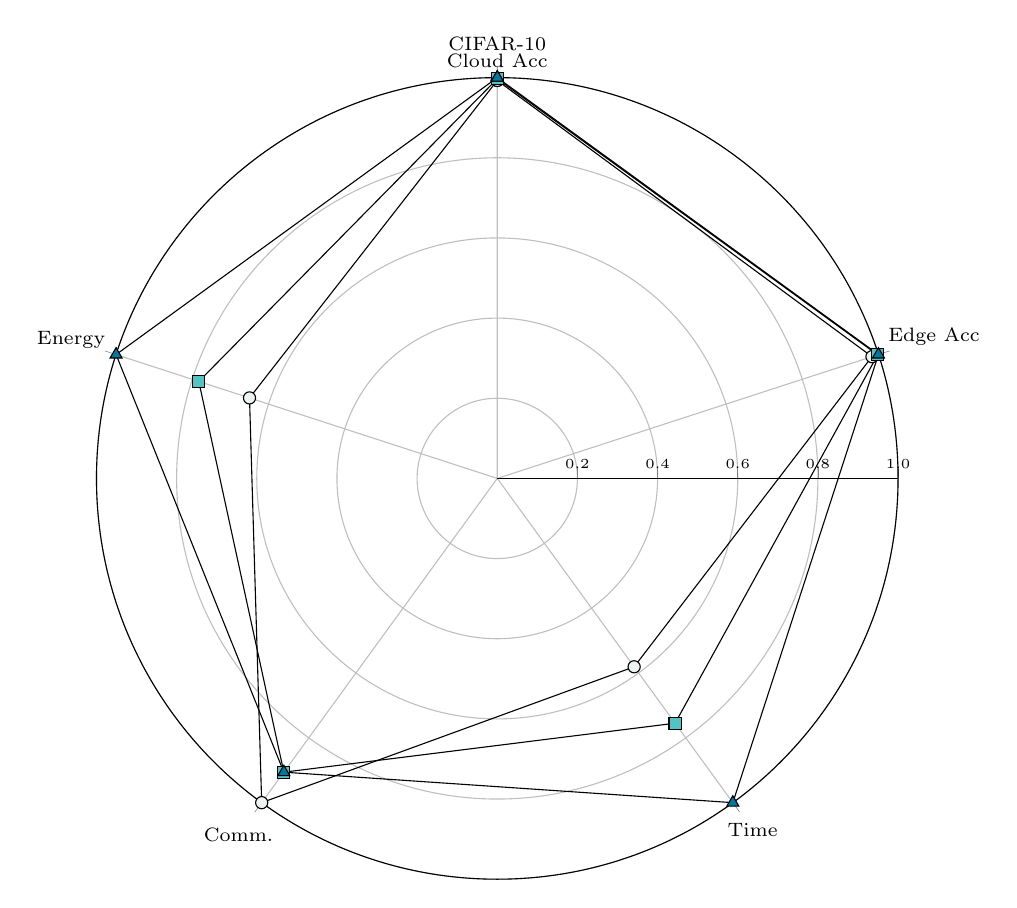
\begin{tikzpicture}
\begin{polaraxis}[
    width=0.97\linewidth,
    ymin=0, ymax=1,
    ytick={0.2,0.4,0.6,0.8,1.0},
    yticklabels={0.2,0.4,0.6,0.8,1.0},
    xtick={90,18,306,234,162},
    xticklabels={Cloud Acc,Edge Acc,Time,Comm.,Energy},
    clip=false,
    grid=both,
    title={CIFAR-10},
    title style={font=\scriptsize, yshift=-0.8em},
    tick label style={font=\scriptsize},
    xticklabel style={font=\scriptsize, align=center},
    yticklabel style={font=\tiny, align=center},
    legend to name=radarlegend,
    legend style={
        draw=none,
        legend columns=0,
        font=\scriptsize
    },
]
\addplot+[
    black,
    mark=*,
    mark size=2.2pt,
    mark options={fill=cbase, draw=black}
] coordinates {
    (90,0.993) (18,0.983) (306,0.581) (234,1.000) (162,0.650) (90,0.993)
};
\addlegendentry{H-FedAvg}

\addplot+[
    black,
    mark=square*,
    mark size=2.2pt,
    mark options={fill=cwo, draw=black}
] coordinates {
    (90,0.997) (18,0.998) (306,0.755) (234,0.906) (162,0.783) (90,0.997)
};
\addlegendentry{EdgeQGFed w/o RS}

\addplot+[
    black,
    mark=triangle*,
    mark size=2.5pt,
    mark options={fill=cmain, draw=black}
] coordinates {
    (90,1.000) (18,1.000) (306,1.000) (234,0.906) (162,1.000) (90,1.000)
};
\addlegendentry{EdgeQGFed}
\end{polaraxis}
\end{tikzpicture}

\vspace{0.2em}
{\scriptsize (a)}
\end{minipage}
\hfill
\begin{minipage}{0.241\textwidth}
\centering
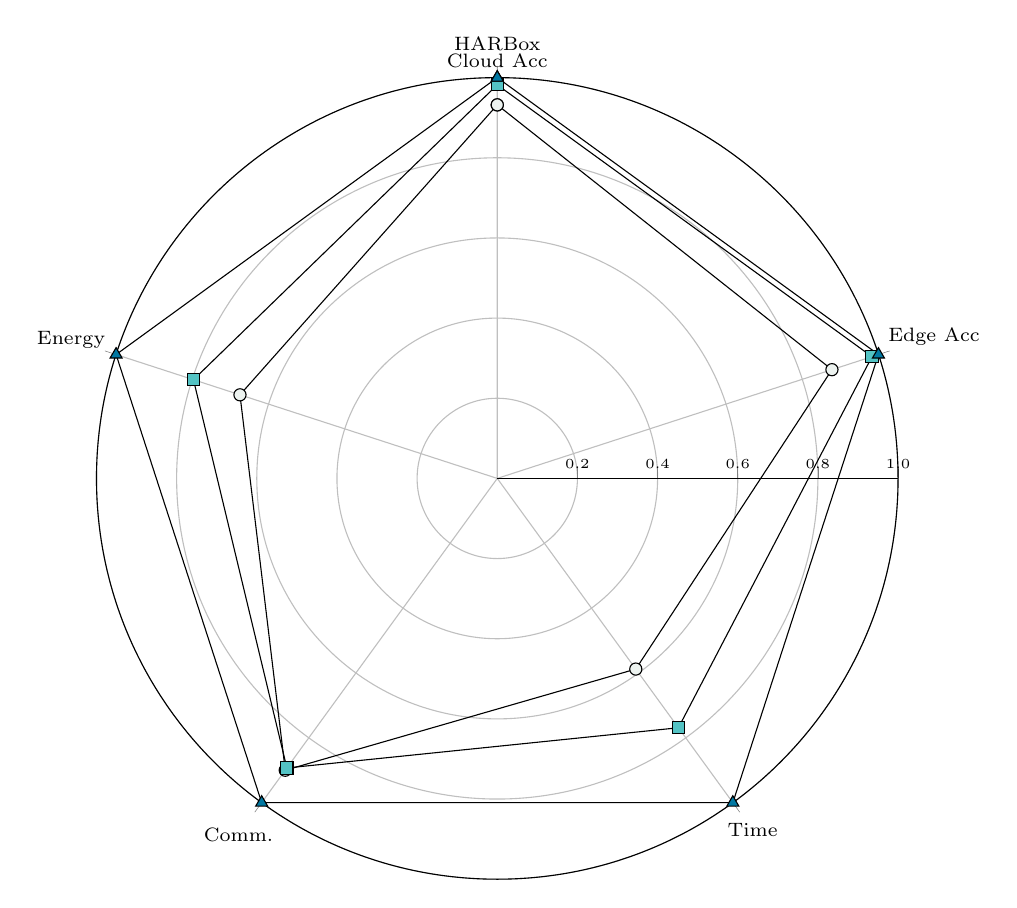
\begin{tikzpicture}
\begin{polaraxis}[
    width=0.97\linewidth,
    ymin=0, ymax=1,
    ytick={0.2,0.4,0.6,0.8,1.0},
    yticklabels={0.2,0.4,0.6,0.8,1.0},
    xtick={90,18,306,234,162},
    xticklabels={Cloud Acc,Edge Acc,Time,Comm.,Energy},
    clip=false,
    grid=both,
    title={HARBox},
    title style={font=\scriptsize, yshift=-0.8em},
    tick label style={font=\scriptsize},
    xticklabel style={font=\scriptsize, align=center},
    yticklabel style={font=\tiny, align=center},
]
\addplot+[
    black,
    mark=*,
    mark size=2.2pt,
    mark options={fill=cbase, draw=black},
    forget plot
] coordinates {
    (90,0.932) (18,0.878) (306,0.588) (234,0.900) (162,0.675) (90,0.932)
};

\addplot+[
    black,
    mark=square*,
    mark size=2.2pt,
    mark options={fill=cwo, draw=black},
    forget plot
] coordinates {
    (90,0.982) (18,0.983) (306,0.769) (234,0.893) (162,0.797) (90,0.982)
};

\addplot+[
    black,
    mark=triangle*,
    mark size=2.5pt,
    mark options={fill=cmain, draw=black},
    forget plot
] coordinates {
    (90,1.000) (18,1.000) (306,1.000) (234,1.000) (162,1.000) (90,1.000)
};
\end{polaraxis}
\end{tikzpicture}

\vspace{0.2em}
{\scriptsize (b)}
\end{minipage}

\vspace{-2em}
\ref{radarlegend}

% \vspace{-0.3em}
\caption{Radar comparison of model performance and system efficiency on (a) CIFAR-10 and (b) HARBox. Time, communication, and energy are reversely normalized so that larger values indicate better efficiency.}
\label{fig:radar_ablation}
\end{figure}
\section{Preliminaries and Problem Formulation}
\label{sec:preliminaries}

\subsection{云边端协同系统}

本文考虑一个云边端协同学习系统，包括一个云服务器、一组边缘服务器 $\mathcal{E}=\{1,\ldots,E\}$ 和一组客户端设备 $\mathcal{C}=\{1,\ldots,C\}$。每个客户端 $i$ 关联到一个边缘服务器 $e(i)\in\mathcal{E}$。客户端拥有本地数据集
\begin{equation}
    \mathcal{D}_i=\mathcal{D}_i^l\cup\mathcal{D}_i^u,
\end{equation}
其中 $\mathcal{D}_i^l$ 和 $\mathcal{D}_i^u$ 分别表示有标签数据和无标签数据。

为适应跨模态边缘任务，样本 $x$ 可以来自不同数据形态，包括图像、传感序列和网络流量特征。本文使用统一的特征抽象表示不同输入。设 $f_\phi(\cdot)$ 为编码器，$h_{\theta_e}(\cdot)$ 为边缘服务器 $e$ 上的分类器，$h_{\theta_c}(\cdot)$ 为云端教师分类器。对于图像任务，$f_\phi$ 可由预训练轻量视觉编码器实现；对于传感序列和网络流量特征，$f_\phi$ 可以为恒等映射或轻量特征变换，由边缘分类器直接处理结构化特征。训练过程中主要更新边缘分类器和云端教师分类器，客户端不承担复杂模型训练。

\subsection{通信预算与时延目标}

在第 $t$ 轮训练中，系统选择客户端集合 $\mathcal{S}_t\subseteq\mathcal{C}$ 参与训练，活跃边缘服务器集合为 $\mathcal{E}_t$。每轮通信预算约束为
\begin{equation}
    \sum_{i\in\mathcal{S}_t} m_i^{\mathrm{ce}}
    + \sum_{e\in\mathcal{E}_t} m_e^{\mathrm{ec}}
    + \sum_{e\in\mathcal{E}_t} m_e^{\mathrm{ceg}}
    \le B_t ,
    \label{eq:budget}
\end{equation}
其中 $m_i^{\mathrm{ce}}$ 表示客户端到边缘的上传量，$m_e^{\mathrm{ec}}$ 表示边缘到云端的上传量，$m_e^{\mathrm{ceg}}$ 表示云端到边缘的下发量，$B_t$ 为第 $t$ 轮通信预算。

本文将每轮时延建模为
\begin{equation}
    T_t = T_t^{\mathrm{c2e}}
        + T_t^{\mathrm{edge}}
        + T_t^{\mathrm{e2c}}
        + T_t^{\mathrm{cloud}}
        + T_t^{\mathrm{c2e\_down}},
    \label{eq:latency}
\end{equation}
其中 $T_t^{\mathrm{c2e}}$ 为端到边上传时延，$T_t^{\mathrm{edge}}$ 为边缘训练时延，$T_t^{\mathrm{e2c}}$ 为边到云上传时延，$T_t^{\mathrm{cloud}}$ 为云端聚合时延，$T_t^{\mathrm{c2e\_down}}$ 为云到边下发时延。除最终性能外，本文还关注 time-to-target accuracy，即模型首次达到目标精度所需的累计系统时延。

\section{EdgeQGFed 方法}
\label{sec:method}

本节给出 EdgeQGFed 的完整训练过程。EdgeQGFed 不是让客户端直接训练模型，而是将客户端、边缘服务器和云端分别承担不同职责。客户端负责提供被选中的数据或轻量特征；边缘服务器接收其覆盖范围内的客户端数据，并执行主要模型更新；云端不再简单平均边缘模型，而是根据边缘上传的质量摘要建模边缘节点关系，生成个性化边缘更新和全局教师模型。

在第 $t$ 轮训练中，EdgeQGFed 先在客户端层进行资源感知采样，得到参与集合 $\mathcal{S}_t$。随后，每个活跃边缘服务器 $e$ 从其关联客户端集合中接收一个批次数据，利用有标签样本进行监督学习，利用无标签样本进行云边一致性学习和伪标签学习。边缘服务器完成若干步更新后，将模型更新、类别原型和训练质量信号组成摘要 $s_e$ 上传给云端。云端基于这些摘要构建质量感知图，通过图注意力计算边缘节点之间的知识共享权重，并将个性化参数下发给对应边缘服务器。下面按照这一轮训练的实际发生顺序展开说明。

EdgeQGFed 的整体流程如图~\ref{fig:fig1} 所示。图中自下而上对应客户端采样、边缘训练和云端图聚合，自上而下对应云端向边缘服务器下发个性化更新。

\begin{figure*}[t]
    \centering
    \IfFileExists{fig1.pdf}
    {\includegraphics[width=0.8\textwidth]{fig1.pdf}}
    {\fbox{\parbox{0.78\textwidth}{\centering 图~\ref{fig:fig1} 占位：云端质量感知图注意力、边缘半监督训练和客户端资源感知采样。}}}
    \caption{EdgeQGFed 云边端协同学习框架。客户端层执行资源感知采样，边缘层执行半监督训练与摘要构建，云端通过质量感知图注意力实现跨边缘知识协调。}
    \label{fig:fig1}
\end{figure*}

\subsection{资源感知客户端采样}
\label{subsec:sampling}

每轮训练首先要决定哪些客户端参与。若仅随机选择客户端，系统可能把通信预算消耗在低带宽、高掉线或数据贡献较低的设备上。为此，EdgeQGFed 为客户端 $i$ 定义资源感知效用：
\begin{equation}
    U_i =
    \frac{
    \eta_l l_i + \eta_d d_i + \eta_b b_i^{\mathrm{up}} + \eta_a a_i
    }
    {(T_i^{\mathrm{up}})^{\eta_t}},
    \label{eq:client_utility}
\end{equation}
其中 $l_i$ 表示有标签比例，$d_i$ 表示归一化数据规模，$b_i^{\mathrm{up}}$ 表示归一化上行带宽，$a_i=1-p_i^{\mathrm{drop}}$ 表示客户端可用性，$T_i^{\mathrm{up}}$ 表示估计上传时延。$\eta_l$、$\eta_d$、$\eta_b$、$\eta_a$ 和 $\eta_t$ 分别控制数据质量、数据规模、链路带宽、可用性和时延代价的影响。

系统按照 $U_i$ 对候选客户端排序，并在每个边缘服务器的并行上传限制和式~\eqref{eq:budget} 的通信预算下选择 $\mathcal{S}_t$。这样做的目的不是单纯选择数据最多的客户端，而是在有限通信资源下优先选择“数据有价值且链路代价可接受”的参与者。

\subsection{边缘侧半监督训练}
\label{subsec:edge_training}

完成客户端采样后，边缘服务器 $e$ 接收其关联的活跃客户端批次 $\mathcal{B}_e=\mathcal{B}_e^l\cup\mathcal{B}_e^u$。其中 $\mathcal{B}_e^l$ 为有标签样本，$\mathcal{B}_e^u$ 为无标签样本。边缘服务器首先通过编码器得到样本表示 $z=f_\phi(x)$，再由边缘分类器 $h_{\theta_e}$ 输出预测。对有标签样本，基本监督损失为
\begin{equation}
    \mathcal{L}_{\mathrm{sup}}^e =
    \frac{1}{|\mathcal{B}_e^l|}
    \sum_{(x,y)\in\mathcal{B}_e^l}
    \ell_{\mathrm{ce}}\left(h_{\theta_e}(f_\phi(x)), y\right).
    \label{eq:sup_loss}
\end{equation}

对于 NSL-KDD 这类类别高度不均衡的网络流量任务，少数类样本在整体准确率中贡献较小，普通交叉熵容易偏向 Normal 和 DoS 等多数类。因此，本文在该类任务中使用类别均衡监督损失：
\begin{equation}
    \mathcal{L}_{\mathrm{sup}}^e =
    \frac{1}{|\mathcal{B}_e^l|}
    \sum_{(x,y)\in\mathcal{B}_e^l}
    \omega_y \ell_{\mathrm{ce}}\left(h_{\theta_e}(f_\phi(x)), y\right),
    \label{eq:weighted_sup_loss}
\end{equation}
其中 $\omega_y$ 为类别 $y$ 的权重。设有标签样本中类别 $k$ 的计数为 $n_k$，类别权重定义为
\begin{equation}
    \omega_k =
    \mathrm{clip}\left(
    \frac{
    \left(\frac{1}{K}\sum_{j=1}^{K}n_j\right)^{\alpha_w}
    }{
    (n_k+\epsilon)^{\alpha_w}
    },
    \omega_{\min}, \omega_{\max}
    \right),
    \label{eq:class_weight}
\end{equation}
其中 $K$ 为类别数，$\alpha_w$ 控制重加权强度，$\omega_{\min}$ 和 $\omega_{\max}$ 防止权重过小或过大。该设计只在类别不均衡任务中启用，用于提升 macro-F1 和少数类 recall。

由于边缘侧通常只有少量标签，无标签样本也需要被利用。EdgeQGFed 使用云端教师模型指导边缘学生模型。给定弱增强样本 $a_w(x)$ 和强增强样本 $a_s(x)$，边缘模型和云端教师模型分别输出
\begin{align}
    p_e &= \mathrm{softmax}\left(h_{\theta_e}(f_\phi(a_s(x)))/T_p\right), \nonumber\\
    p_c &= \mathrm{softmax}\left(h_{\theta_c}(f_\phi(a_w(x)))/T_p\right),
    \label{eq:edge_cloud_pred}
\end{align}
其中 $T_p$ 为伪标签温度。边缘模型应在强增强下与云端教师在弱增强下保持一致，因此一致性损失为
\begin{equation}
    \mathcal{L}_{\mathrm{con}}^e =
    d(p_e,p_c),
    \label{eq:consistency_loss}
\end{equation}
其中 $d(\cdot,\cdot)$ 可取均方误差、$\ell_1$ 距离或 KL 散度。训练早期预测不稳定时，EdgeQGFed 可通过置信度门控只对可靠样本计算一致性损失。

仅使用一致性约束仍然不能明确给出无标签样本的类别监督。为此，EdgeQGFed 进一步使用置信度加权伪标签。设 $\hat{y}_e=\arg\max p_e$，$\hat{y}_c=\arg\max p_c$，$q_e=\max p_e$，$q_c=\max p_c$。只有当边缘预测和云端预测一致时，无标签样本才被用于伪标签训练，其权重为
\begin{equation}
    w(x) =
    \mathbf{1}[\hat{y}_e=\hat{y}_c]
    \cdot
    \sigma\left(\frac{q_e-\tau_e}{\gamma}\right)
    \cdot
    \sigma\left(\frac{q_c-\tau_c}{\gamma}\right),
    \label{eq:pseudo_weight}
\end{equation}
其中 $\tau_e$ 和 $\tau_c$ 分别为边缘和云端置信度阈值，$\gamma$ 为平滑温度。对应的伪标签损失为
\begin{equation}
    \mathcal{L}_{\mathrm{pl}}^e =
    \frac{\sum_{x\in\mathcal{B}_e^u} w(x)
    \ell_{\mathrm{ce}}\left(h_{\theta_e}(f_\phi(a_s(x))), \hat{y}_c\right)}
    {\sum_{x\in\mathcal{B}_e^u} w(x)+\epsilon}.
    \label{eq:pseudo_loss}
\end{equation}

最终，边缘服务器 $e$ 的训练目标为
\begin{equation}
    \mathcal{L}_e =
    \mathcal{L}_{\mathrm{sup}}^e
    + \lambda_t \mathcal{L}_{\mathrm{con}}^e
    + \lambda_p \mathcal{L}_{\mathrm{pl}}^e,
    \label{eq:edge_loss}
\end{equation}
其中 $\lambda_t$ 通过 warm-up 逐步增大，$\lambda_p$ 控制伪标签损失权重。对于网络流量五分类任务，伪标签启动更晚且阈值更高，以避免多数类高置信伪标签过早压制 R2L、U2R 等少数类。

\subsection{少标签与类别不均衡处理}
\label{subsec:stratified_label}

在少标签设置下，若每个客户端随机选择有标签样本，少数类可能在训练中几乎不可见。EdgeQGFed 因此在类别不均衡任务中使用分层标注采样。对于客户端 $i$ 的本地索引集合 $\mathcal{I}_i$，其标注预算为
\begin{equation}
    L_i=\min\left(|\mathcal{I}_i|,\max(\lfloor r|\mathcal{I}_i|\rfloor,L_{\min})\right),
    \label{eq:label_budget}
\end{equation}
其中 $r$ 为标签比例，$L_{\min}$ 为每个客户端最小标注数。系统先从客户端本地可见类别中尽量保留代表性有标签样本，再用随机样本补齐预算。该策略不改变总体标签比例，只提升有标签样本的类别覆盖度。

进一步地，对于 NSL-KDD 五分类任务，训练批次中会保留一部分有标签样本并按类别权重重复抽样，使 R2L、U2R 等少数类在边缘监督训练中出现得更频繁。该增强只作用于训练采样过程，不改变测试集分布，因此更适合用 macro-F1、macro recall 和每类 recall 评估其效果。

\subsection{边缘摘要构建}
\label{subsec:summary}

边缘服务器完成本地更新后，不向云端上传原始数据，而是上传能够反映模型状态和训练质量的边缘摘要：
\begin{equation}
    s_e = \{\theta_e, P_e, n_e, \rho_e, r_e, c_e, b_e\}.
    \label{eq:summary}
\end{equation}
其中 $\theta_e$ 表示边缘上传的聚合对象，$P_e$ 为类别原型矩阵，$n_e$ 为各类别原型计数，$\rho_e$ 为平均伪标签权重，$r_e$ 为有标签样本比例，$c_e$ 为平均云端置信度，$b_e$ 为本轮处理样本数。

类别原型用于描述边缘节点当前看到的数据语义。对于类别 $k$，原型定义为
\begin{equation}
    P_e^k =
    \frac{1}{|\mathcal{B}_{e,k}^l|}
    \sum_{(x,y)\in\mathcal{B}_{e,k}^l} f_\phi(x),
    \label{eq:prototype}
\end{equation}
其中 $\mathcal{B}_{e,k}^l$ 表示边缘服务器 $e$ 当前批次中属于类别 $k$ 的有标签样本集合。若某个类别在当前边缘批次中不存在，则该类别原型计数为零，并在云端聚合时降低其贡献。通过上传摘要而非原始数据，EdgeQGFed 在保留跨边缘知识协调所需信息的同时降低通信和隐私开销。

\subsection{云端质量感知图注意力聚合}
\label{subsec:graph_aggregation}

云端接收活跃边缘摘要后，需要判断哪些边缘节点之间更适合共享知识。直接平均所有边缘更新会忽略数据分布、标签质量和伪标签可靠性的差异。EdgeQGFed 将活跃边缘节点视为图中的节点，并根据边缘摘要构造质量感知图。

对于边缘节点 $e$，云端从模型参数提取模型签名 $u_e$，从类别原型提取原型签名 $v_e$。对于两个活跃边缘节点 $i$ 和 $j$，注意力得分为
\begin{align}
    a_{ij} =
    &\ \mathrm{cos}(u_i,u_j)
    + \alpha_p \mathrm{cos}(v_i,v_j)
    + \alpha_q (1-|\rho_i-\rho_j|) \nonumber \\
    &+ \alpha_r (1-|r_i-r_j|)
    + \alpha_c (1-|c_i-c_j|)
    + \beta \mathbf{1}[i=j],
    \label{eq:attention_score}
\end{align}
其中模型签名和原型签名刻画边缘节点的语义相似性，$\rho_i$、$r_i$ 和 $c_i$ 分别反映伪标签质量、标签比例和预测置信度。$\alpha_p$、$\alpha_q$、$\alpha_r$ 和 $\alpha_c$ 控制不同质量信号的贡献，$\beta$ 为自连接偏置，用于保留边缘节点自身知识。

云端随后对注意力得分进行归一化，得到图注意力矩阵：
\begin{equation}
    A_{ij} =
    \frac{\exp(a_{ij}/\tau_g)}
    {\sum_{k\in\mathcal{E}_t}\exp(a_{ik}/\tau_g)},
    \label{eq:attention_matrix}
\end{equation}
其中 $\tau_g$ 为图注意力温度。$A_{ij}$ 越大，表示边缘节点 $i$ 在生成自身个性化模型时越应吸收来自边缘节点 $j$ 的知识。因此，云端为每个目标边缘节点生成个性化参数
\begin{equation}
    \tilde{\theta}_i =
    \sum_{j\in\mathcal{E}_t} A_{ij}\theta_j.
    \label{eq:personalized_param}
\end{equation}

除了个性化边缘参数，云端还需要维护全局教师模型。EdgeQGFed 根据边缘处理样本数和伪标签质量计算全局聚合权重：
\begin{equation}
    \bar{\theta} =
    \sum_{i\in\mathcal{E}_t}
    \omega_i \tilde{\theta}_i,
    \quad
    \omega_i =
    \frac{b_i(\rho_i+1)}
    {\sum_{j\in\mathcal{E}_t} b_j(\rho_j+1)}.
    \label{eq:global_param}
\end{equation}
若采用 AEMA，云端教师模型更新为
\begin{equation}
    \theta_c \leftarrow
    \mu \theta_c + (1-\mu)\bar{\theta},
    \label{eq:ema}
\end{equation}
其中 $\mu$ 为平滑系数。若采用 FedAvg，则直接使用 $\bar{\theta}$ 替换云端教师模型。最后，云端将 $\tilde{\theta}_i$ 下发给对应边缘服务器；对于本轮未得到个性化参数的边缘节点，云端下发全局回退参数，以避免边缘模型长期陈旧。

\begin{algorithm}[t]
\caption{云端质量感知图注意力聚合}
\label{alg:graph_aggregation}
\begin{algorithmic}[1]
\REQUIRE 活跃边缘摘要 $\mathcal{S}^{\mathrm{edge}}_t=\{s_e\}_{e\in\mathcal{E}_t}$，图温度 $\tau_g$，权重系数 $\alpha_p,\alpha_q,\alpha_r,\alpha_c$，自连接偏置 $\beta$
\ENSURE 云端教师模型 $\theta_c$，个性化边缘参数 $\{\tilde{\theta}_e\}_{e\in\mathcal{E}_t}$
\FOR{each active edge $e\in\mathcal{E}_t$}
    \STATE 提取模型签名 $u_e$ 和原型签名 $v_e$
\ENDFOR
\FOR{each pair of active edges $(i,j)$}
    \STATE 根据式~\eqref{eq:attention_score} 计算质量感知得分 $a_{ij}$
\ENDFOR
\STATE 根据式~\eqref{eq:attention_matrix} 得到注意力矩阵 $A$
\FOR{each target edge $i\in\mathcal{E}_t$}
    \STATE 根据式~\eqref{eq:personalized_param} 生成个性化参数 $\tilde{\theta}_i$
\ENDFOR
\STATE 根据式~\eqref{eq:global_param} 和式~\eqref{eq:ema} 更新云端教师模型
\STATE 下发个性化参数或全局回退参数到边缘服务器
\end{algorithmic}
\end{algorithm}

\subsection{整体训练流程}
\label{subsec:procedure}

综合上述步骤，EdgeQGFed 的一轮训练可以概括为“选客户端、边缘训练、上传摘要、云端图聚合、下发更新”。算法~\ref{alg:edgeqgfed} 给出完整流程。该流程体现了本文的核心思想：客户端只轻量参与，边缘服务器承担主要训练，云端利用质量感知图注意力进行跨边缘协同。

\begin{algorithm}[t]
\caption{EdgeQGFed 云边端协同训练流程}
\label{alg:edgeqgfed}
\begin{algorithmic}[1]
\REQUIRE 客户端集合 $\mathcal{C}$，边缘服务器集合 $\mathcal{E}$，云端教师模型 $\theta_c$，边缘模型 $\{\theta_e\}_{e\in\mathcal{E}}$，通信预算 $B_t$，总训练轮数 $T$
\ENSURE 云端教师模型 $\theta_c$，边缘模型 $\{\theta_e\}_{e\in\mathcal{E}}$
\FOR{$t=1$ to $T$}
    \STATE 根据式~\eqref{eq:client_utility} 执行资源感知客户端采样，得到 $\mathcal{S}_t$
    \FOR{each active edge server $e\in\mathcal{E}_t$}
        \STATE 接收关联客户端上传的数据或特征，构造 $\mathcal{B}_e^l$ 和 $\mathcal{B}_e^u$
        \STATE 根据式~\eqref{eq:sup_loss} 或式~\eqref{eq:weighted_sup_loss} 计算监督损失
        \STATE 根据式~\eqref{eq:consistency_loss} 和式~\eqref{eq:pseudo_loss} 计算无标签损失
        \STATE 根据式~\eqref{eq:edge_loss} 更新边缘模型 $\theta_e$
        \IF{满足云端聚合间隔}
            \STATE 根据式~\eqref{eq:summary} 构建并上传边缘摘要 $s_e$
        \ENDIF
    \ENDFOR
    \IF{云端收到边缘摘要}
        \STATE 调用算法~\ref{alg:graph_aggregation} 执行质量感知图注意力聚合
        \STATE 更新云端教师模型，并下发个性化边缘参数
    \ENDIF
\ENDFOR
\end{algorithmic}
\end{algorithm}

\section{实验评估}
\label{sec:evaluation}

本节从跨模态学习性能和网络系统效率两个角度评估 EdgeQGFed。实验重点不是证明某一数据集上的最高集中式精度，而是验证该框架在图像、传感序列和网络流量任务中，能否在少标签、non-IID、通信受限和客户端不稳定参与条件下保持有效。除跨模态总体性能实验外，系统开销、鲁棒性和消融实验仅选择代表性数据集进行分析，以避免重复展示相同趋势。

\subsection{实验设置}
\label{subsec:exp_setup}

\textbf{数据集与任务。}
本文使用四个公开数据集进行评估，覆盖图像、传感序列和网络流量三类边缘智能任务。CIFAR-10 和 CIFAR-100 用于评估图像任务下的表征迁移与类别扩展能力；HARBox 用于评估用户级传感序列数据上的边缘协同学习；NSL-KDD 用于评估网络流量任务。对于 CIFAR-10 和 CIFAR-100，本文采用 Dirichlet non-IID 划分，并重点报告 $\alpha=0.3$ 和 $\alpha=0.1$；HARBox 按用户划分。

对于 NSL-KDD，本文首先对连续特征进行归一化，并将协议、服务和连接状态等离散字段编码为数值特征。原始二分类设置通常将所有攻击合并为 Attack，该任务在预实验中准确率可接近 $99\%$，难以充分反映边缘节点之间的攻击类型差异。为避免该任务过于饱和，本文将其转换为 Normal、DoS、Probe、R2L 和 U2R 五分类任务，并按客户端级 non-IID 方式划分。该设置更适合评估个性化边缘模型，因为不同边缘节点可能面对不同攻击组合，简单全局平均容易偏向多数类，而个性化更新能够更直接地反映局部流量分布。

\begin{table}[t]
\centering
\caption{数据集与默认划分设置}
\label{tab:datasets}
\begin{tabular}{lcccc}
\toprule
数据集 & 数据形态 & 类别数 & 划分方式 & 标签比例 \\
\midrule
 CIFAR-10 & 图像 & 10 & Dirichlet & 0.1 \\
 CIFAR-100 & 图像 & 100 & Dirichlet & 0.1 \\
HARBox & 传感器时序 & 5 & 用户级划分 & 0.1 \\
NSL-KDD & 网络流量 & 5 & Dirichlet & 0.1 \\
\bottomrule
\end{tabular}
\end{table}

\textbf{系统配置。}
默认系统包含一个云服务器、多个边缘服务器和若干客户端。图像任务默认设置为 4 个边缘服务器和 128 个客户端；HARBox 和 NSL-KDD 默认设置为 5 个边缘服务器和 100 个客户端。每轮训练中，云端根据采样策略选择部分客户端，活跃客户端将当前批次数据或特征上传到对应边缘服务器。默认链路采用异构 edge profile，并在系统实验中进一步改变通信预算、带宽分布和客户端掉线率。

\textbf{对比方法。}
总体性能实验比较 EdgeQGFed 与多类代表性联邦学习方法，包括同步聚合、近端正则、异步更新、缓冲式聚合、个性化联邦学习和图结构个性化方法。系统效率和消融实验则聚焦于少量关键对照，包括 H-FedAvg、H-FedAvg+PL、EdgeQGFed w/o Graph、EdgeQGFed w/o RS、EdgeQGFed w/o PL 和完整 EdgeQGFed，以分析本文各模块的贡献。

\textbf{评价指标。}
学习性能使用云端准确率和边缘平均准确率衡量。对于 NSL-KDD，本文额外记录 macro-F1，以避免总体准确率掩盖少数类性能。系统效率使用总通信量、累计通信量、形式化轮时延、累计估计时延和 time-to-target accuracy 衡量。为解释系统行为，本文还记录选中客户端数、活跃客户端数、客户端掉线率、伪标签比例、伪标签权重和图注意力统计量。

\subsection{跨模态总体性能}
\label{subsec:overall_performance}

首先在四个数据集上比较 EdgeQGFed 与现有代表性联邦学习方法。该实验用于回答框架是否能适配不同数据形态，而不是只在单一图像任务上有效。表~\ref{tab:overall_performance} 采用横向大表形式报告不同数据集和划分设置下的云端准确率；对于 NSL-KDD，同时记录五分类准确率和 macro-F1。图~\ref{fig:overall} 展示不同数据集上的准确率收敛曲线。

\begin{table*}[t]
\centering
\caption{跨模态边缘任务下与现有方法的总体性能对比}
\label{tab:overall_performance}
\resizebox{\textwidth}{!}{
\begin{tabular}{lccccccc}
\toprule
方法 & CIFAR-10 & CIFAR-10 & CIFAR-100 & CIFAR-100 & HARBox & NSL-KDD & NSL-KDD \\
& Dir(0.3) & Dir(0.1) & Dir(0.3) & Dir(0.1) & Real-world & Acc. & Macro-F1 \\
\midrule
FedAvg & \rule{0.8cm}{0.4pt} & \rule{0.8cm}{0.4pt} & \rule{0.8cm}{0.4pt} & \rule{0.8cm}{0.4pt} & \rule{0.8cm}{0.4pt} & \rule{0.8cm}{0.4pt} & \rule{0.8cm}{0.4pt} \\
FedProx & \rule{0.8cm}{0.4pt} & \rule{0.8cm}{0.4pt} & \rule{0.8cm}{0.4pt} & \rule{0.8cm}{0.4pt} & \rule{0.8cm}{0.4pt} & \rule{0.8cm}{0.4pt} & \rule{0.8cm}{0.4pt} \\
FedAsync & \rule{0.8cm}{0.4pt} & \rule{0.8cm}{0.4pt} & \rule{0.8cm}{0.4pt} & \rule{0.8cm}{0.4pt} & \rule{0.8cm}{0.4pt} & \rule{0.8cm}{0.4pt} & \rule{0.8cm}{0.4pt} \\
FedBuff & \rule{0.8cm}{0.4pt} & \rule{0.8cm}{0.4pt} & \rule{0.8cm}{0.4pt} & \rule{0.8cm}{0.4pt} & \rule{0.8cm}{0.4pt} & \rule{0.8cm}{0.4pt} & \rule{0.8cm}{0.4pt} \\
FedAC & \rule{0.8cm}{0.4pt} & \rule{0.8cm}{0.4pt} & \rule{0.8cm}{0.4pt} & \rule{0.8cm}{0.4pt} & \rule{0.8cm}{0.4pt} & \rule{0.8cm}{0.4pt} & \rule{0.8cm}{0.4pt} \\
ASAFL & \rule{0.8cm}{0.4pt} & \rule{0.8cm}{0.4pt} & \rule{0.8cm}{0.4pt} & \rule{0.8cm}{0.4pt} & \rule{0.8cm}{0.4pt} & \rule{0.8cm}{0.4pt} & \rule{0.8cm}{0.4pt} \\
FedAMP & \rule{0.8cm}{0.4pt} & \rule{0.8cm}{0.4pt} & \rule{0.8cm}{0.4pt} & \rule{0.8cm}{0.4pt} & \rule{0.8cm}{0.4pt} & \rule{0.8cm}{0.4pt} & \rule{0.8cm}{0.4pt} \\
pFedGraph & \rule{0.8cm}{0.4pt} & \rule{0.8cm}{0.4pt} & \rule{0.8cm}{0.4pt} & \rule{0.8cm}{0.4pt} & \rule{0.8cm}{0.4pt} & \rule{0.8cm}{0.4pt} & \rule{0.8cm}{0.4pt} \\
FedSaC & \rule{0.8cm}{0.4pt} & \rule{0.8cm}{0.4pt} & \rule{0.8cm}{0.4pt} & \rule{0.8cm}{0.4pt} & \rule{0.8cm}{0.4pt} & \rule{0.8cm}{0.4pt} & \rule{0.8cm}{0.4pt} \\
FedAMP-Async & \rule{0.8cm}{0.4pt} & \rule{0.8cm}{0.4pt} & \rule{0.8cm}{0.4pt} & \rule{0.8cm}{0.4pt} & \rule{0.8cm}{0.4pt} & \rule{0.8cm}{0.4pt} & \rule{0.8cm}{0.4pt} \\
pFedGraph-Async & \rule{0.8cm}{0.4pt} & \rule{0.8cm}{0.4pt} & \rule{0.8cm}{0.4pt} & \rule{0.8cm}{0.4pt} & \rule{0.8cm}{0.4pt} & \rule{0.8cm}{0.4pt} & \rule{0.8cm}{0.4pt} \\
EdgeQGFed & \rule{0.8cm}{0.4pt} & \rule{0.8cm}{0.4pt} & \rule{0.8cm}{0.4pt} & \rule{0.8cm}{0.4pt} & \rule{0.8cm}{0.4pt} & \rule{0.8cm}{0.4pt} & \rule{0.8cm}{0.4pt} \\
\bottomrule
\end{tabular}
}
\end{table*}

\textbf{绘图方式。}
图~\ref{fig:overall}(a) 为折线图，横轴为训练步数，纵轴为云端准确率，不同曲线表示四个数据集；图~\ref{fig:overall}(b) 为折线图，横轴为累计通信量，纵轴为云端准确率，不同曲线表示主要方法；图~\ref{fig:overall}(c) 为分组柱状图，横轴为数据集，纵轴为 time-to-target。

\subsection{通信效率与时延}
\label{subsec:comm_efficiency}

随后评估通信预算、三层时延和系统能耗对训练效率的影响。该实验更贴近 INFOCOM 关注的网络系统问题，即在有限通信资源下，方法是否能够以更低通信量、更短系统时延和更少能耗达到目标精度。为减少重复，本文选择 HARBox 和 CIFAR-10 作为代表性任务，分别覆盖传感序列与图像数据。通信预算分别设置为 HARBox 的 $\{50,100,200,300\}$ MB 和 CIFAR-10 的 $\{50,100,300,600\}$ MB。表~\ref{tab:budget_energy} 给出假设结果，用于说明后续实验记录格式。

\begin{table*}[t]
\centering
\caption{通信预算、时延与能耗敏感性（假设结果）}
\label{tab:budget_energy}
\resizebox{\textwidth}{!}{
\begin{tabular}{llcccccc}
\toprule
数据集 & 方法 & Round Budget & 云端准确率 & 边缘准确率 & Time-to-Target & 每轮通信量 & Energy-to-Target \\
& & (MB) & (\%) & (\%) & (s) & (MB) & (J) \\
\midrule
HARBox & H-FedAvg & 100 & 75.42 & 73.86 & 31.45 & 16.82 & 14.27 \\
HARBox & H-FedAvg+PL & 100 & 78.36 & 76.91 & 24.06 & 16.95 & 12.08 \\
HARBox & EdgeQGFed & 100 & 83.29 & 81.74 & 18.50 & 15.14 & 9.63 \\
CIFAR-10 & H-FedAvg & 100 & 84.38 & 82.47 & 39.80 & 30.00 & 26.72 \\
CIFAR-10 & H-FedAvg+PL & 100 & 87.64 & 85.91 & 30.64 & 30.00 & 22.18 \\
CIFAR-10 & EdgeQGFed & 100 & 90.12 & 88.96 & 23.12 & 30.00 & 17.36 \\
\bottomrule
\end{tabular}
}
\end{table*}

\textbf{绘图方式。}
图~\ref{fig:comm_latency_energy}(a) 为折线图，横轴为累计通信量，纵轴为云端准确率，不同曲线表示 H-FedAvg、H-FedAvg+PL 和 EdgeQGFed。图~\ref{fig:comm_latency_energy}(b) 为堆叠柱状图，横轴为方法，纵轴为摊销每轮时延，分解为端到边上传、边缘计算、边到云上传、云端聚合和云到边下发五个部分。图~\ref{fig:comm_latency_energy}(c) 为堆叠柱状图，横轴为方法，纵轴为每轮能耗，分解为通信能耗和计算能耗。能耗由日志中的时延分量离线计算，例如端到边上传能耗为 $E^{\mathrm{c2e}}=P_{\mathrm{client}}T^{\mathrm{c2e}}$，边缘计算能耗为 $E^{\mathrm{edge}}=P_{\mathrm{edge}}T^{\mathrm{edge}}$。

\subsection{链路异构与客户端移动性}
\label{subsec:heterogeneity}

本文进一步评估带宽异构和客户端不稳定参与下的鲁棒性。该实验主要在 HARBox 上进行，因为其用户级划分更接近移动边缘设备持续参与的场景。本文改变客户端掉线率、带宽分布和移动性模式，以验证资源感知采样能否避开低质量链路客户端，以及图注意力聚合能否在边缘更新不完整时保持稳定。

\begin{table}[t]
\centering
\caption{链路异构与客户端移动性下的鲁棒性（假设结果）}
\label{tab:mobility}
\begin{tabular}{lcccc}
\toprule
场景 & 方法 & 云端准确率 & 活跃客户端数 & Time-to-Target \\
\midrule
Static & H-FedAvg & 75.42 & 40.0 & 31.45 \\
Static & EdgeQGFed w/o RS & 80.37 & 40.0 & 23.86 \\
Static & EdgeQGFed & 83.29 & 40.0 & 18.50 \\
Mobility & H-FedAvg & 68.74 & 28.6 & 47.32 \\
Mobility & EdgeQGFed w/o RS & 74.18 & 29.1 & 35.74 \\
Mobility & EdgeQGFed & 80.46 & 33.8 & 24.92 \\
\bottomrule
\end{tabular}
\end{table}

\textbf{绘图方式。}
图~\ref{fig:mobility}(a) 为折线图，横轴为客户端掉线率，纵轴为云端准确率，不同曲线表示 H-FedAvg、EdgeQGFed w/o RS 和 EdgeQGFed。图~\ref{fig:mobility}(b) 为点线图，横轴为带宽异构模式，纵轴为 Time-to-Target。图~\ref{fig:mobility}(c) 为双轴柱线图，横轴为掉线率，左轴为活跃客户端数，右轴为预算使用率，用于解释资源感知采样在移动性条件下的作用。

\subsection{消融实验}
\label{subsec:ablation}

为了分析各组件的作用，本文分别去除图注意力聚合、资源感知采样、伪标签学习和云边一致性训练。消融实验默认在 HARBox 和 CIFAR-10 上进行，分别代表传感序列任务和图像任务。该实验同时报告准确率、Time-to-Target、通信量和能耗，从性能与效率两个角度解释 EdgeQGFed 的收益来源。

\begin{table*}[t]
\centering
\caption{组件消融结果（假设结果）}
\label{tab:ablation}
\resizebox{\textwidth}{!}{
\begin{tabular}{llccccc}
\toprule
数据集 & 变体 & 云端准确率 & 边缘准确率 & Time-to-Target & 每轮通信量 & Energy-to-Target \\
& & (\%) & (\%) & (s) & (MB) & (J) \\
\midrule
HARBox & Full EdgeQGFed & 81.58 & 80.12 & 18.50 & 15.14 & 9.63 \\
HARBox & w/o Graph & 79.42 & 77.96 & 20.84 & 15.10 & 10.38 \\
HARBox & w/o Resource Sampling & 80.06 & 78.73 & 23.76 & 17.82 & 12.61 \\
HARBox & w/o Pseudo Label & 77.85 & 76.44 & 27.13 & 14.96 & 13.40 \\
HARBox & w/o Consistency & 78.62 & 77.18 & 25.48 & 15.02 & 12.92 \\
CIFAR-10 & Full EdgeQGFed & 90.60 & 89.47 & 23.12 & 30.00 & 17.36 \\
CIFAR-10 & w/o Graph & 89.12 & 87.76 & 26.44 & 29.96 & 18.84 \\
CIFAR-10 & w/o Resource Sampling & 89.74 & 88.21 & 29.06 & 32.54 & 21.37 \\
CIFAR-10 & w/o Pseudo Label & 87.46 & 86.03 & 34.85 & 29.88 & 24.92 \\
CIFAR-10 & w/o Consistency & 88.25 & 86.91 & 31.72 & 29.92 & 23.40 \\
\bottomrule
\end{tabular}
}
\end{table*}

\textbf{绘图方式。}
图~\ref{fig:ablation}(a) 为分组柱状图，横轴为消融变体，纵轴为云端准确率，分组为 HARBox 和 CIFAR-10。图~\ref{fig:ablation}(b) 为雷达图，维度包括 Accuracy、Time-to-Target、Communication、Energy 和 Robustness，其中越小越好的指标先归一化并反向处理。

\subsection{统计异质性与少标签敏感性}
\label{subsec:sensitivity}

本文进一步分析 EdgeQGFed 在不同 non-IID 强度和标签稀缺程度下的稳定性。对于 CIFAR-10 和 CIFAR-100，本文改变 Dirichlet 参数 $\alpha\in\{0.1,0.3,0.5,1.0\}$，其中较小的 $\alpha$ 表示更强的数据异构性。对于 HARBox，本文改变标签比例 $\{0.05,0.1,0.2,1.0\}$，考察少标签传感序列任务中的半监督收益。

\begin{table}[t]
\centering
\caption{异质性与标签比例敏感性（假设结果）}
\label{tab:sensitivity}
\begin{tabular}{llccc}
\toprule
数据集 & 变量 & 取值 & 云端准确率 & 边缘准确率 \\
\midrule
CIFAR-10 & $\alpha$ & 0.1 & 90.60 & 89.47 \\
CIFAR-10 & $\alpha$ & 0.3 & 91.34 & 90.08 \\
CIFAR-10 & $\alpha$ & 0.5 & 91.82 & 90.51 \\
CIFAR-10 & $\alpha$ & 1.0 & 92.15 & 90.84 \\
CIFAR-100 & $\alpha$ & 0.1 & 59.42 & 58.37 \\
CIFAR-100 & $\alpha$ & 0.3 & 61.08 & 60.11 \\
HARBox & 标签比例 & 0.05 & 77.36 & 75.82 \\
HARBox & 标签比例 & 0.1 & 81.58 & 80.12 \\
HARBox & 标签比例 & 0.2 & 84.06 & 82.47 \\
HARBox & 标签比例 & 1.0 & 89.14 & 87.62 \\
\bottomrule
\end{tabular}
\end{table}

\textbf{绘图方式。}
图~\ref{fig:sensitivity}(a) 为折线图，横轴为 Dirichlet 参数，纵轴为云端准确率，曲线为 CIFAR-10 和 CIFAR-100。图~\ref{fig:sensitivity}(b) 为折线图，横轴为有标签比例，纵轴为云端准确率，展示 HARBox 在少标签条件下的性能变化。

\subsection{质量感知图注意力机制分析}
\label{subsec:graph_analysis}

为解释云端图注意力是否真正依据边缘节点质量进行选择性聚合，本文记录图注意力对角权重、伪标签可靠性和预测置信度等统计量。表~\ref{tab:graph_signal} 给出假设结果。需要注意的是，CIFAR-100 类别数更多，原始置信度不宜与 CIFAR-10 直接比较，因此本文额外给出归一化置信度。

\begin{table}[t]
\centering
\caption{质量感知图信号统计（假设结果）}
\label{tab:graph_signal}
\begin{tabular}{lcccc}
\toprule
数据集 & 注意力对角 & 可靠性 & 置信度 & 归一化置信度 \\
\midrule
CIFAR-10 & 0.44 & 0.80 & 0.96 & 0.956 \\
CIFAR-100 & 0.53 & 0.55 & 0.75 & 0.747 \\
HARBox & 0.46 & 0.63 & 0.98 & 0.975 \\
NSL-KDD & 0.44 & 0.80 & 0.94 & 0.925 \\
\bottomrule
\end{tabular}
\end{table}

\textbf{绘图方式。}
图~\ref{fig:graph_analysis}(a) 为热力图，横轴为源边缘节点，纵轴为目标边缘节点，颜色表示注意力权重。图~\ref{fig:graph_analysis}(b) 为散点图，横轴为边缘可靠性，纵轴为被分配的注意力权重，用于观察高质量边缘节点是否获得更多知识共享权重。

\subsection{NSL-KDD 少数类识别分析}
\label{subsec:nslkdd_detail}

网络流量五分类任务存在明显类别不均衡，仅报告整体准确率可能掩盖 R2L 和 U2R 等少数类识别不足。为此，本文进一步报告每类 recall 和 macro-F1。该实验用于证明类别均衡监督与分层标注采样能够提升少数类识别能力。

\begin{table}[t]
\centering
\caption{NSL-KDD 五分类详细结果（假设结果）}
\label{tab:nslkdd_detail}
\resizebox{\columnwidth}{!}{
\begin{tabular}{lccccccc}
\toprule
方法 & Acc & Macro-F1 & Normal & DoS & Probe & R2L & U2R \\
\midrule
H-FedAvg & 78.64 & 0.512 & 0.93 & 0.88 & 0.61 & 0.24 & 0.18 \\
H-FedAvg+PL & 81.37 & 0.574 & 0.94 & 0.90 & 0.66 & 0.31 & 0.25 \\
EdgeQGFed & 85.92 & 0.681 & 0.96 & 0.92 & 0.73 & 0.46 & 0.38 \\
\bottomrule
\end{tabular}
}
\end{table}

\textbf{绘图方式。}
图~\ref{fig:nslkdd_recall} 为分组柱状图，横轴为五个类别，纵轴为 recall，不同柱表示 H-FedAvg、H-FedAvg+PL 和 EdgeQGFed。

\subsection{可扩展性分析}
\label{subsec:scalability}

最后，本文分析客户端规模扩大时 EdgeQGFed 的通信和时延开销是否可控。该实验主要在 CIFAR-10 上进行，将客户端数从 128 扩展到 1000。对于更大规模的 10000 客户端，本文仅作为系统模拟设定讨论，因为此时每个 logical client 更接近数据分片而非真实用户。

\begin{table}[t]
\centering
\caption{客户端规模扩展性（假设结果）}
\label{tab:scalability}
\begin{tabular}{lccccc}
\toprule
数据集 & 客户端数 & 每轮客户端 & 云端准确率 & Time-to-Target & 每轮通信量 \\
\midrule
CIFAR-10 & 128 & 32 & 90.60 & 23.12 & 30.00 \\
CIFAR-10 & 256 & 32 & 90.18 & 24.06 & 30.00 \\
CIFAR-10 & 500 & 64 & 89.74 & 26.88 & 60.00 \\
CIFAR-10 & 1000 & 64 & 89.21 & 28.34 & 60.00 \\
\bottomrule
\end{tabular}
\end{table}

\textbf{绘图方式。}
图~\ref{fig:scalability} 为双轴折线图，横轴为客户端规模，左轴为 Time-to-Target，右轴为云端准确率，用于展示大规模逻辑客户端下的效率与性能变化。

\section{Conclusion}
本文提出 EdgeQGFed，一种面向跨模态边缘智能任务的通信高效云-边-端协同学习框架。该框架将主要训练负载上移至边缘服务器，使弱客户端以轻量方式参与数据贡献；云端进一步利用质量感知图注意力机制建模边缘节点之间的语义相关性和更新可靠性，从而实现选择性知识共享。为适应真实边缘网络，EdgeQGFed 结合资源感知客户端采样、边缘侧半监督学习和三层通信时延建模，在通信预算、链路异构和客户端不稳定参与条件下同时优化模型性能和训练效率。实验设计覆盖图像、传感序列和网络流量任务，并从总体性能、time-to-accuracy、通信时延、系统能耗、鲁棒性、组件消融、少数类识别和可扩展性等方面验证方法有效性。未来工作将进一步研究更大规模边缘拓扑下的异步协同训练，以及面向更复杂任务类型的自适应模型部署策略。

% \bibliographystyle{IEEEtran}
% % argument is your BibTeX string definitions and bibliography database(s)
% \bibliography{IEEEabrv, EdgeQGFed.bib}

\end{document}
